\phantomsection
\chapter*{Scopo del documento}
\addcontentsline{toc}{chapter}{Scopo del documento}

In questo documento è riporta la descrizione dell’architettura di sistema del progetto Sistema di monitoraggio ambientale usando diagrammi in Unified Modeling Language (UML).
Sulla base dei requisiti di sistema descritti nel documento precedente, è stata creata l'architettura del progetto, qui descritta utilizzando diagrammi di contesto, dei componenti, e BPMN. 

\chapter{Analisi di contesto}

%\begin{itemize}
%    \item activity chart per descrivere registrazione nella descrizione; 
%    \item descrivere bene la registrazione quando si parla del login;
%    \item fare la descrizione utilizzando reference a RF;
%    \item azione dell'utente per visualizzare le schermate: nella descrizione %            inserire le schermate che può visualizzare.
%\end{itemize}

Nel seguente capitolo viene descritto il funzionamento del sistema, attraverso una descrizione testuale e una rappresentazione grafica basata su Context Diagram.

\vspace{5mm} 
Nella seguente parte vengono presentati gli \textbf{attori} e i \textbf{sistemi esterni} con cui l'applicazione "Sistema di monitoraggio ambientale" si interfaccerà.

\section{Utenti e sistemi esterni}
\subsection{Utente}
L'utente è colui che utilizza l'applicazione per visualizzare le informazioni relative alla flora e alla fauna. \\
Il \textbf{RF 2.2} identifica i vari utenti, comune e amministratore, e ne introduce le loro funzionalità.  L'utente comune non ha accesso completo all'applicazione, infatti può selezionare solamente le voci area attiva, fauna, flora e notifiche meteo. Il \textbf{RF 2.4.2} specifica inoltre il funzionamento della guida digitale (flora/fauna). 

\subsection{Amministratore}
L'amministratore è colui che utilizza l'applicazione per monitorare il parco e ricevere le varie notifiche di allerta. \\
Il \textbf{RF 2.2} identifica l'amministratore e le sue funzionalità specificate poi nei \textbf{RF 2.4.1, RF 2.4.3 e 2.5}.

\subsection{Sensori}
Il sistema è utilizzato per fornire dati grezzi sulla situazione ambientale. 

\subsection{Sistema GPS}
Il sistema GPS è utilizzato per fornire dati riguardanti posizione e numero degli animali di medio-grande dimensione.

\subsection{Sistema di calcolo probabilistico}
Il sistema utilizzato per elaborare i dati grezzi forniti dai sensori.

\subsection{Database}
Il database si occupa di salvare tutte le informazioni riguardanti: flora e fauna, storico animali, dati amministratori e probabilità del rischio di avvenimento catastrofi.

\subsection{Sistema di invio mail/notifica}
Il sistema utilizzato per inviare notifiche a utenti, amministratori e autorità locali, come specificato nei \textbf{RF 2.3} e \textbf{RF 2.4.1}.

\pagebreak
\section{Diagramma di contesto}

\begin{figure}[ht]
    \centering
    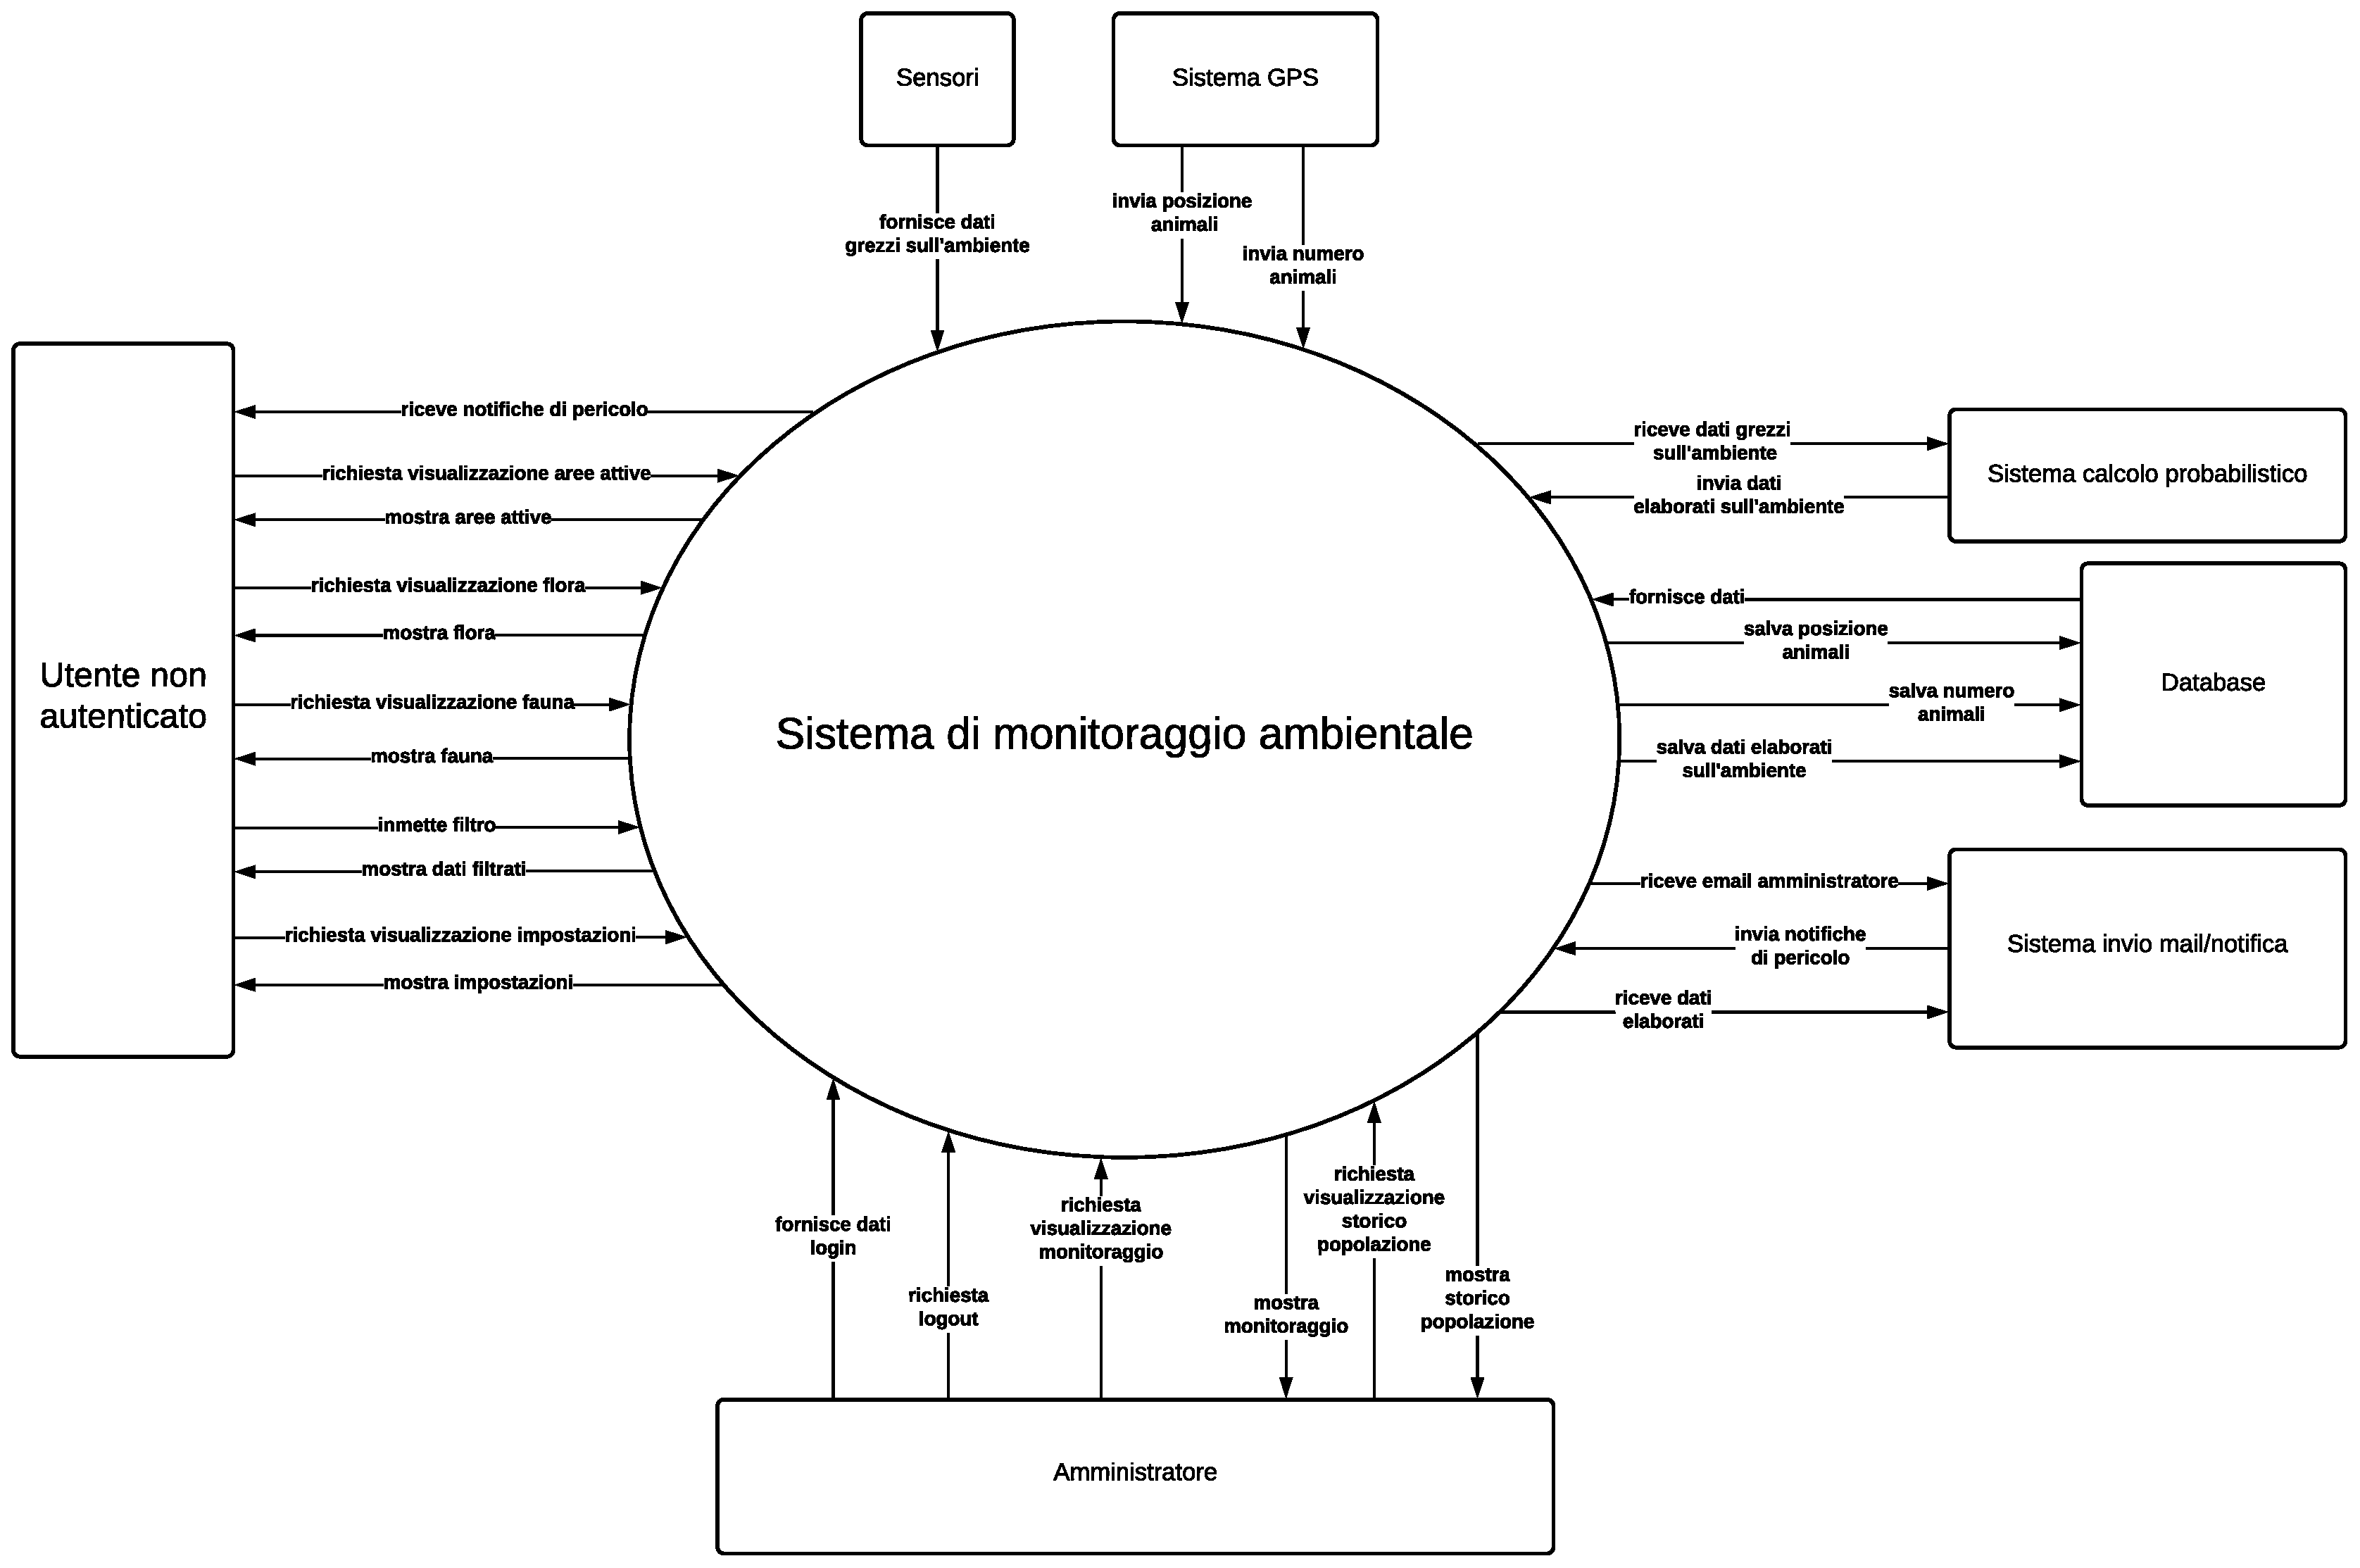
\includegraphics[scale=0.3]{Img/DiagrammaDiContesto.eps}
    \caption{Diagramma di contesto per l'applicazione Sistema di monitoraggio ambientale}
\end{figure}
\vspace{5mm}

\noindent
Nel seguente elenco è possibile trovare una descrizione ad alto livello delle relazioni tra le differenti componenti esterne. \'E bene ricordare che tutti gli scambi di informazioni tra sistemi esterni sono mediati dal \textbf{sistema principale}.
\vspace{5mm}

\noindent
L'\textbf{utente} comune non può eseguire il login e può utilizzare le voci: area attiva, flora, fauna e impostazioni (\textbf{RF 2.2}). Può inoltre impostare un filtro in fauna e flora come descritto nel \textbf{RF 2.4.2}. 

\vspace{5mm}
%\noindent
%L'\textbf{amministratore} deve eseguire la registrazione (\textbf{Figura \ref{fig:reg_amm}}) che non avviene attraverso il sistema, ma deve fornire i dati personali agli sviluppatori. Esso deve dunque effettuare l'autenticazione per poter utilizzare le voci: monitoraggio e storico popolazione come in \textbf{RF 2.2}.

\noindent
L'\textbf{amministratore} deve eseguire la registrazione (\textbf{Figura \ref{fig:reg_amm}}) attraverso gli sviluppatori del sistema, i quali non entrano in contatto con esso in alcun modo e per questo non sono rappresentati del diagramma di contesto. Esso deve dunque effettuare l'autenticazione per poter utilizzare le voci "monitoraggio" e "storico popolazione" come specificato in \textbf{RF 2.2}.

Per effettuare il login, il sistema confronta le credenziali inserite con i dati salvati nel database.

\vspace{5mm}
\noindent
I \textbf{sensori} forniscono i dati grezzi sull'ambiente al sistema che provvederà a salvarli sul database e ad inviarli al sistema di calcolo probabilistico.

\vspace{5mm}
\noindent
Il \textbf{sistema di calcolo probabilistico} invia i dati elaborati al sistema di invio mail/notifiche che, basandosi sui dati ricevuti, invierà i rispettivi messaggi. 

\vspace{5mm}
\noindent
Il \textbf{sistema GPS} fornisce informazioni sulla posizione degli animali e il loro numero. Queste informazioni sono salvate nel database e servono per generare la mappa degli animali e tenere traccia dello storico.

%\begin{figure}[ht]
%    \centering
%    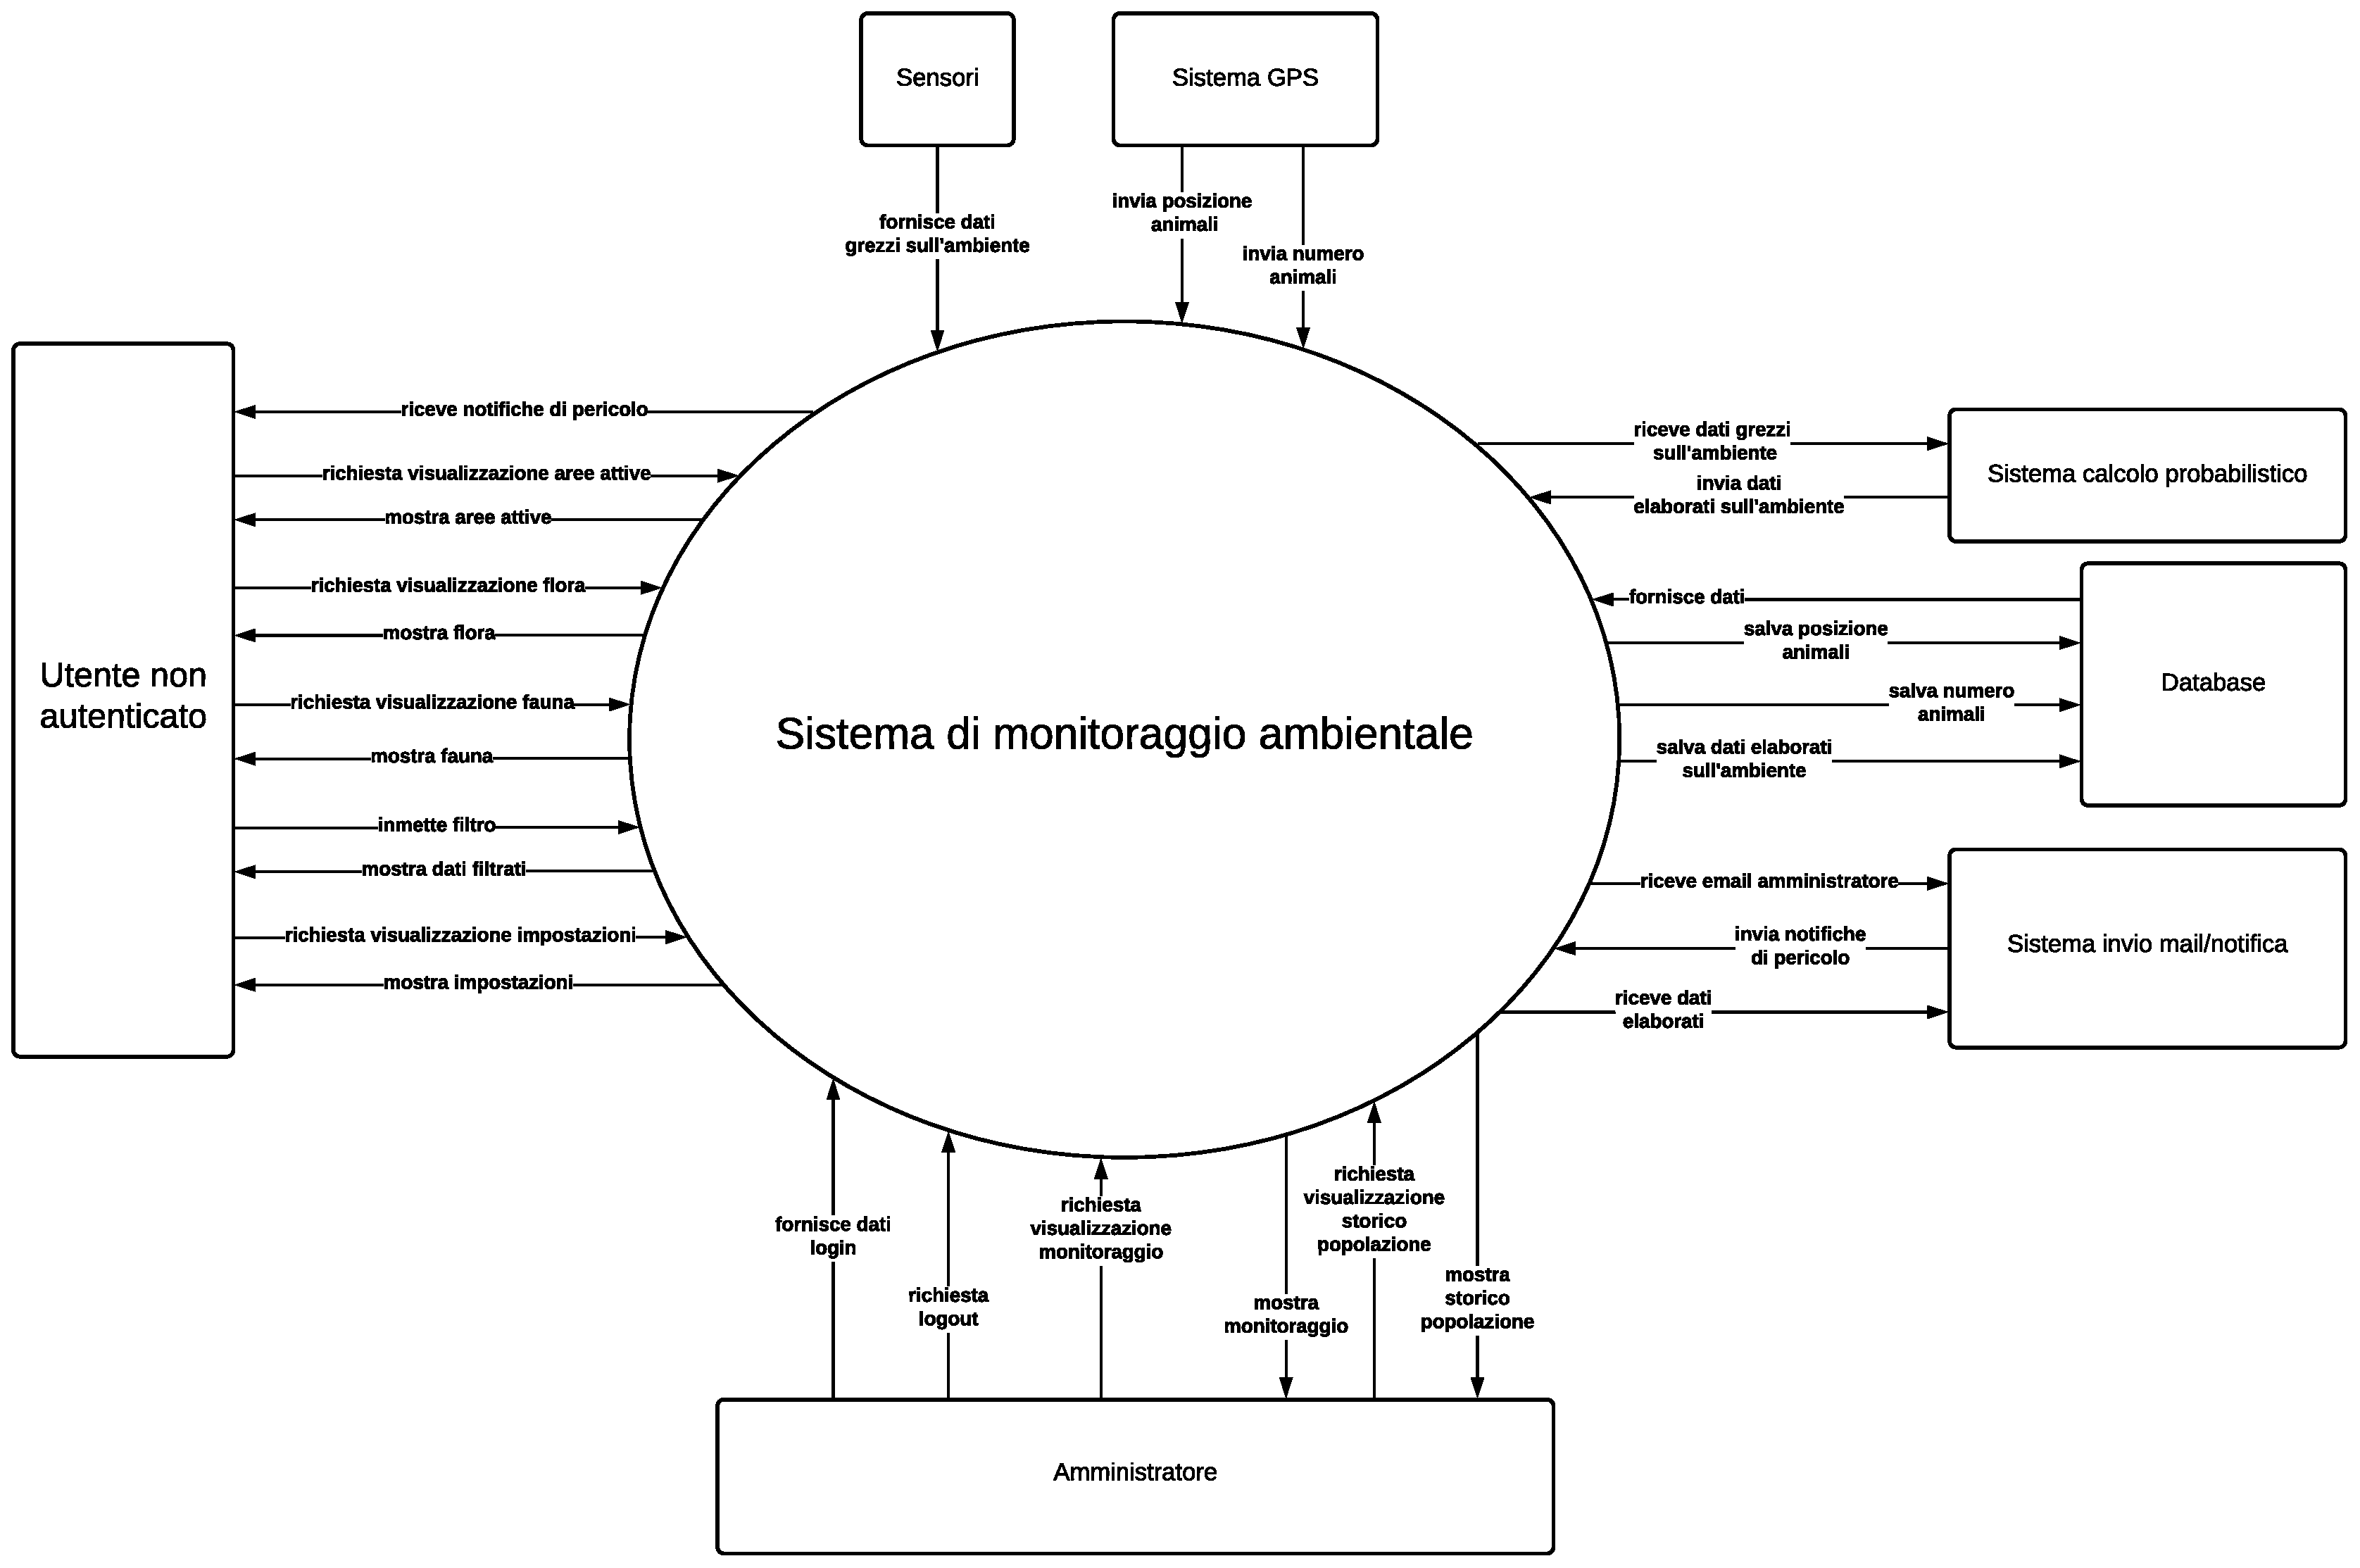
\includegraphics[scale=0.3]{Img/DiagrammaDiContesto.eps}
%    \caption{Diagramma di contesto per l'applicazione Sistema di %monitoraggio ambientale}
%\end{figure}

\begin{figure}[ht]
    \centering
    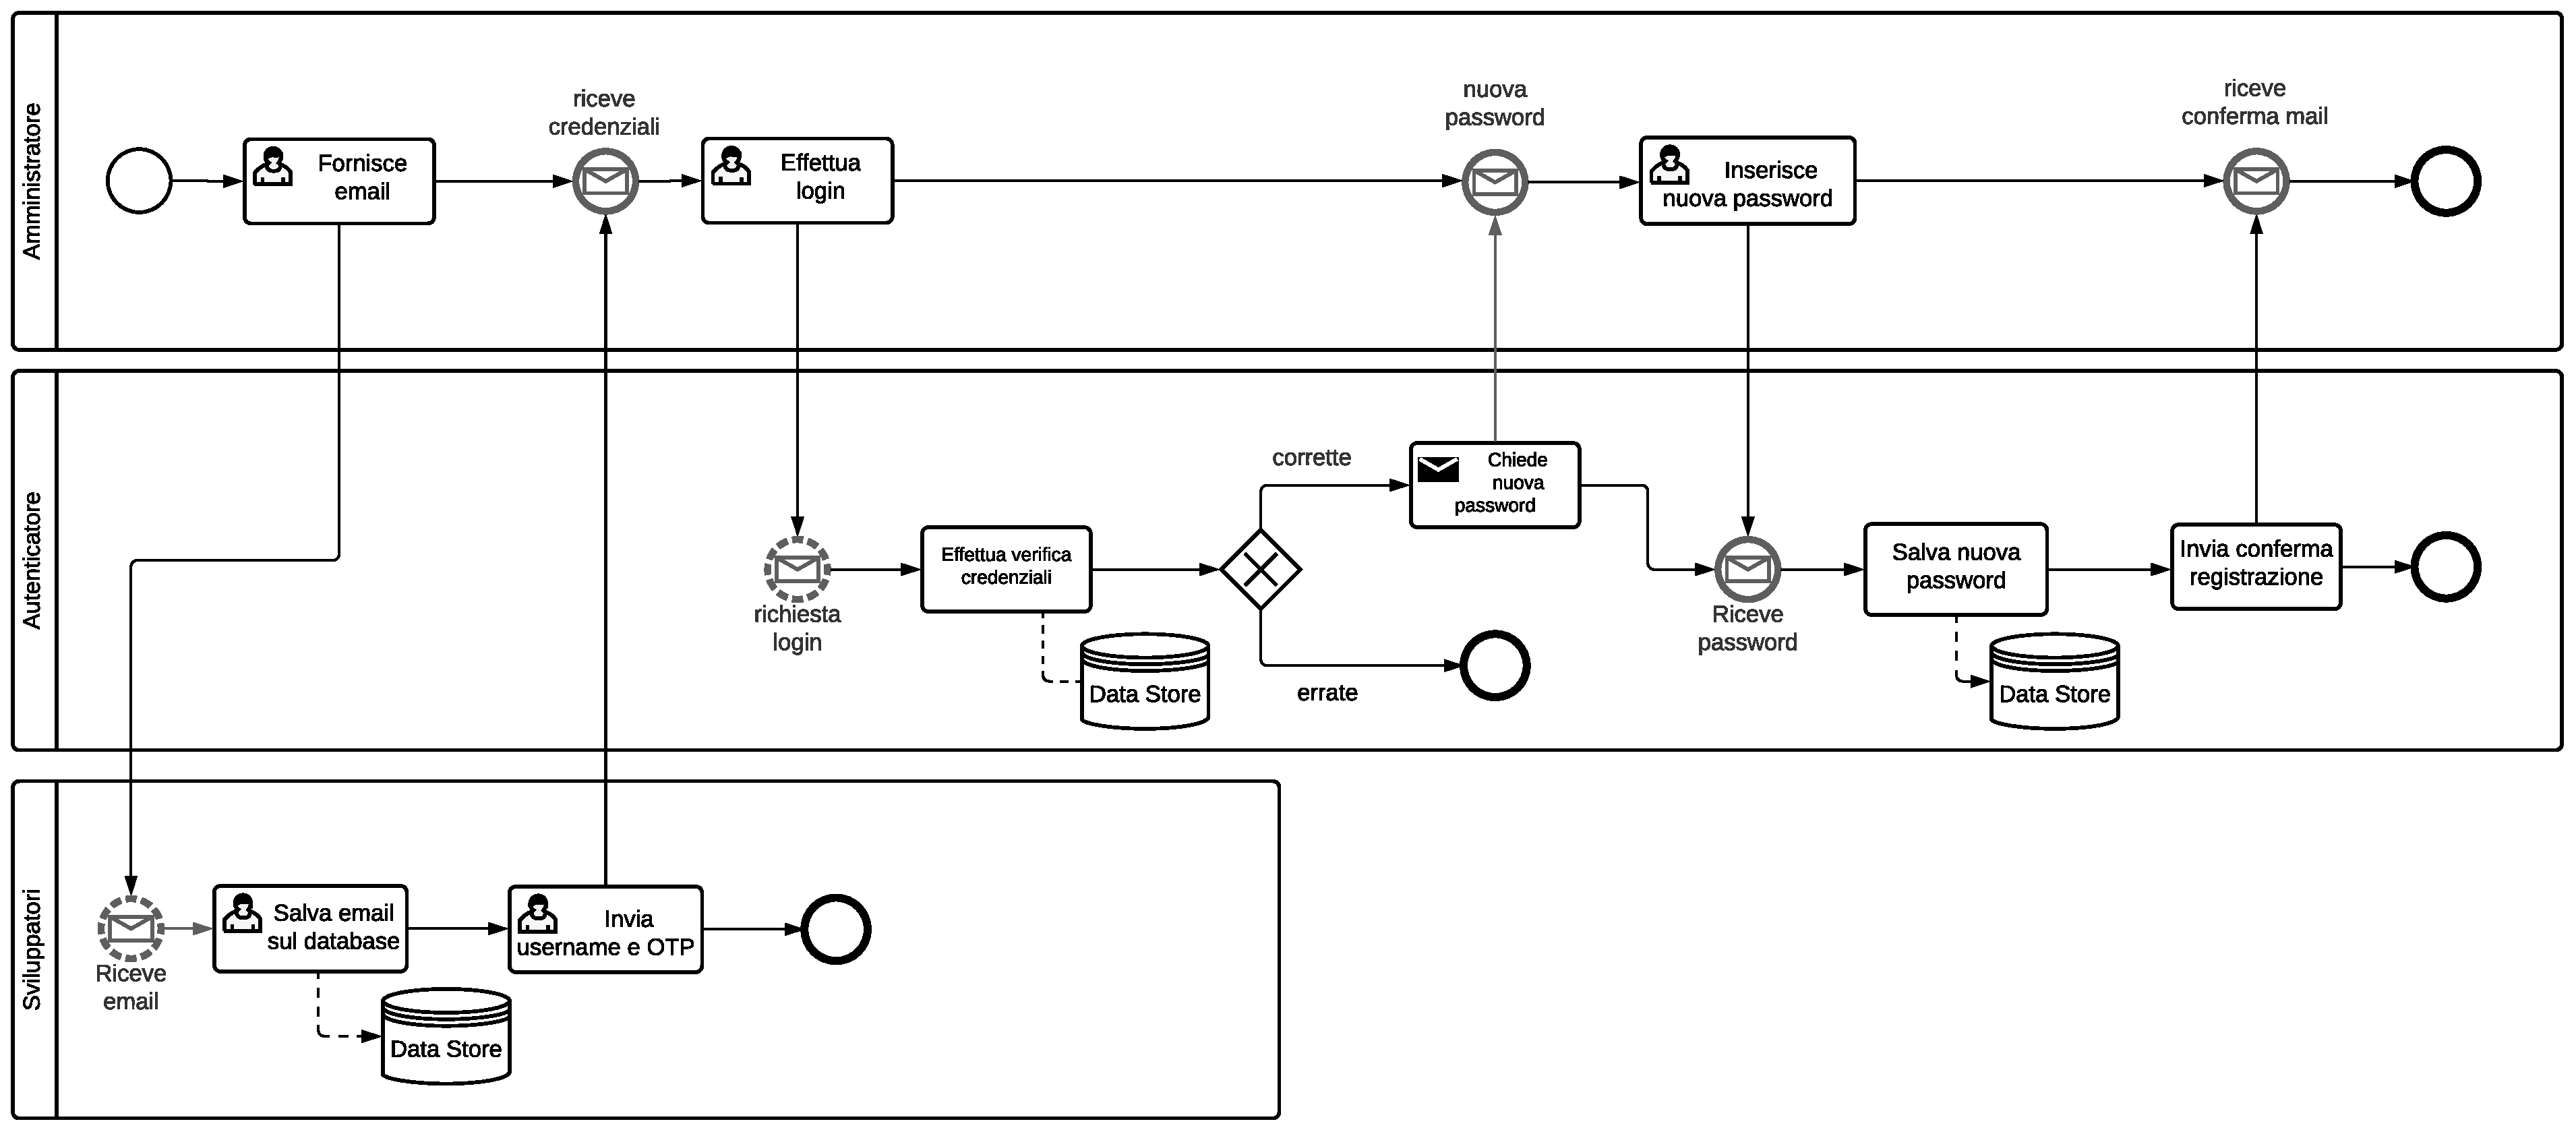
\includegraphics[scale=0.26]{Img/BPMN_reg_amministratore.eps}
    \caption{BPMN Registrazione amministratore}
    \label{fig:reg_amm}
\end{figure}